\chapter{Deployment}

\section{System Architecture}
The deployment architecture is designed to be robust, scalable, and compliant with medical data standards. It follows a decoupled Client-Server model, ensuring separation of concerns between the user interface and the inference logic.

\begin{figure}[h]
    \centering
    % Placeholder for architecture diagram if needed
    \textbf{[Client: Web Browser]} $\longleftrightarrow$ \textbf{[API Gateway / Load Balancer]} $\longleftrightarrow$ \textbf{[Container: FastAPI + Model]}
    \caption{High-Level Deployment Architecture}
\end{figure}

\begin{itemize}
    \item \textbf{Frontend (Client):} A static Single Page Application (SPA) built with HTML5, CSS3 (Glassmorphism design), and vanilla JavaScript. It runs in the user's browser and communicates with the backend via RESTful APIs.
    \item \textbf{Backend (Server):} A high-performance Python application powered by \textbf{FastAPI}. It handles data validation, business logic, and model inference.
    \item \textbf{Model Serving:} The trained models are serialized (using \texttt{joblib}) and embedded within the backend service, ensuring low-latency predictions.
\end{itemize}

\section{Backend Implementation}
The core of the system is the \texttt{Backend} service, designed for asynchronous processing and high throughput.

\subsection{Technology Stack}
\begin{itemize}
    \item \textbf{Framework:} FastAPI (Python 3.9+) for its speed and native support for asynchronous programming.
    \item \textbf{Server:} Uvicorn, an ASGI lightning-fast server implementation.
    \item \textbf{Data Validation:} Pydantic models enforce strict typing on all incoming clinical data, ensuring that invalid inputs (e.g., negative tumor sizes) are rejected before reaching the model.
\end{itemize}

\subsection{API Endpoints}
The backend exposes versioned endpoints to support the clinical workflow:
\begin{itemize}
    \item \texttt{POST /api/v1/cellular/predict}: Accepts WBCD features and returns the diagnosis (Benign/Malignant) with probability scores.
    \item \texttt{POST /api/v1/clinical/triage}: Calculates the risk tier based on clinical rules and model output.
    \item \texttt{GET /api/v1/evaluation/metrics}: Provides real-time access to the current model's performance metrics (Sensitivity, Specificity) for auditing.
\end{itemize}

\section{MLOps \& CI/CD Pipeline}
To maintain clinical safety and reproducibility, we implemented a rigorous MLOps pipeline using \textbf{GitHub Actions} and \textbf{MLflow}.

\subsection{Continuous Integration (CI)}
Every code change triggers an automated workflow defined in \texttt{.github/workflows/ci.yml}:
\begin{enumerate}
    \item \textbf{Linting \& Type Checking:} Code quality is enforced using \texttt{black}, \texttt{isort}, and \texttt{mypy}.
    \item \textbf{Automated Testing:} Unit tests (via \texttt{pytest}) verify the API endpoints and data preprocessing logic.
    \item \textbf{Model Retraining:} The pipeline executes \texttt{run\_train\_wbcd.py} to retrain the model on the latest data.
    \item \textbf{Evaluation Gate:} The script \texttt{run\_evaluate\_wbcd.py} assesses the new model. If the Sensitivity drops below a critical threshold (e.g., 98\%), the pipeline fails, preventing unsafe models from reaching production.
    \item \textbf{Experiment Tracking:}
    \begin{verbatim}
    mlflow ui
    \end{verbatim}
    Launching the MLflow UI allows developers to inspect the metrics and parameters of the training run.
\end{enumerate}

\begin{figure}[H]
    \centering
    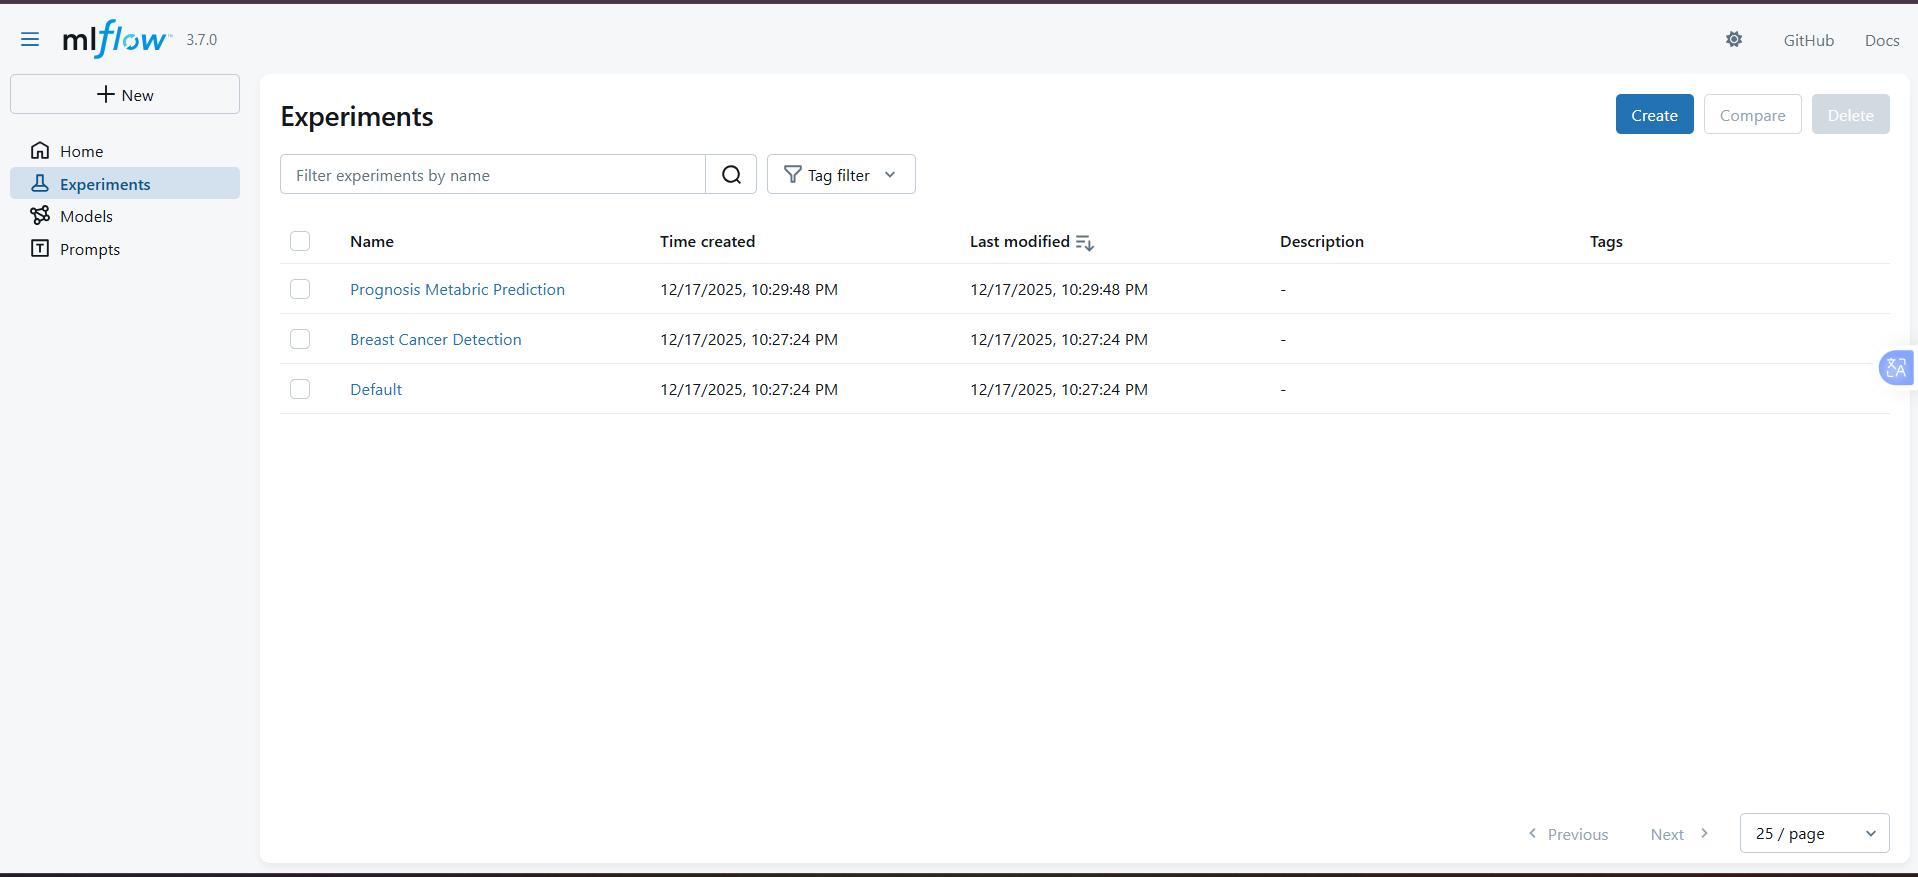
\includegraphics[width=0.9\textwidth]{images/mlflow.png}
    \caption{MLflow Experiment Tracking Dashboard}
\end{figure}

\subsection{Model Registry \& Artifacts}
Successful runs produce immutable artifacts:
\begin{itemize}
    \item \textbf{Model Binaries:} \texttt{.joblib} files for the trained models and scalers.
    \item \textbf{Explainability Data:} \texttt{shap\_explainability.json} containing global feature importance.
    \item \textbf{Performance Reports:} \texttt{roc\_curves.json} and confusion matrices.
\end{itemize}
These artifacts are archived and versioned, allowing full traceability of which model version was active at any given time.



\section{Evidence-Based Deployment Logic}
A unique feature of this deployment is the \textbf{Dynamic Guideline Injection}.
Instead of hard-coding clinical rules, the system loads them from a \texttt{medical\_guidelines.json} file and a \texttt{deployment\_manifest.json} at runtime.

\begin{itemize}
    \item \textbf{Agility:} Clinical thresholds (e.g., the probability cutoff for a biopsy recommendation) can be updated in the JSON configuration without recompiling the code.
    \item \textbf{Compliance:} The \texttt{deployment\_manifest.json} explicitly states the version of the medical guidelines (e.g., NCCN v3.2023) the system is currently using, ensuring regulatory transparency.
\end{itemize}

\section{Clinical Interface (Frontend)}
The web interface is designed for rapid clinical use, prioritizing accessibility and clarity. It features:
\begin{itemize}
    \item \textbf{Smart Triage Dashboard:} Automatically sorts patients by urgency (Critical, High, Medium, Low) based on the backend's risk stratification.
    \item \textbf{Real-time Feedback:} As the clinician enters data, the UI provides immediate visual cues to highlight abnormal values.
    \item \textbf{Interpretation:} It displays the SHAP values (received from the backend) to explain \textit{why} a specific risk score was assigned.
    \item \textbf{Octobre Rose Edition UI:} A completely redesigned interface featuring:
    \begin{itemize}
        \item \textbf{Glassmorphism Design:} A modern, translucent aesthetic for better readability.
        \item \textbf{Inspirational Elements:} Animated quotes (e.g., "Hope is stronger than fear") to support the emotional well-being of the medical staff and patients.
        \item \textbf{Accessibility:} Support for Dark/Light modes to reduce eye strain during long shifts.
    \end{itemize}
\end{itemize}


